\chapter{BIPEDAL WALKING BY TWIN DELAYED DEEP DETERMINISTIC POLICY GRADIENTS}
\label{chap:exp_setup}

\section{Details of the Environment}

\textit{Bipedal-Walker-v3} and \textit{Bipedal-Walker-Hardocore-v3} are simulation environments of a bipedal robot, with relatively flat course and obstacle course respectively. Dynamics of the robot are exactly identical in both environments. Components of the hardcore environment is visualized in \figref{fig:bipedal_hardcore_components}.

\begin{figure}
	\centering
	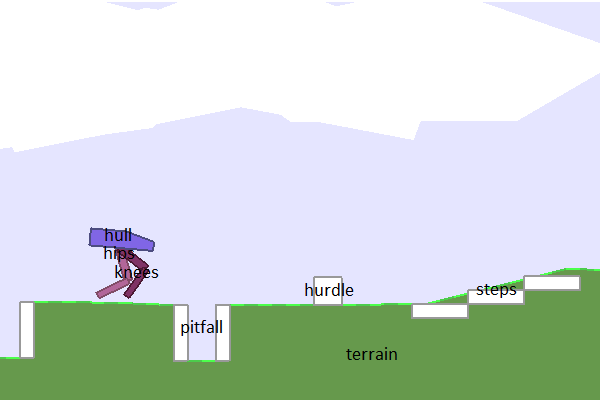
\includegraphics[width=0.95\textwidth]{figures/bipedal/bipedal_annotated.png}
	\caption{Bipedal Walker Hardcore Components}
	\label{fig:bipedal_hardcore_components}
\end{figure}

The robot has kinematic and lidar sensors. It is modeled as Markov Decision Process with deterministic dynamics. 

\textbf{Observation Space}: Hull angle, hull angular velocity, translational velocity on two dimension, joint positions, joint angular speeds, leg ground concats and 10 lidar rangefinder measurements. Details are summarized at Table \ref{table:bpw_obs_space}

\begin{table}[h!]
	\begin{center}
	\begin{tabular}{cccc}
		\textbf{Num} & \textbf{Observation} & \textbf{Interval} \\
		\hline 
		0  & Hull Angle & $[-\pi,\pi]$ \\
		1  & Hull Angular Speed & $[-\infty,\infty]$ \\
		2  & Velocity x & $[-1,1]$ \\
		3  & Velocity y &$[-1,1]$ \\
		4  & Hip 1 Joint Angle & $[-\infty,\infty]$ \\
		5  & Hip 1 Joint Speed & $[-\infty,\infty]$ \\
		6  & Knee 1 Joint Angle & $[-\infty,\infty]$ \\
		7  & Knee 1 Joint Speed & $[-\infty,\infty]$ \\
		8  & Leg 1 Ground Contact Flag & $\{0,1\}$ \\
		9  & Hip 2 Joint Angle & $[-\infty,\infty]$ \\
		10  & Hip 2 Joint Speed & $[-\infty,\infty]$ \\
		11  & Knee 2 Joint Angle & $[-\infty,\infty]$ \\
		12  & Knee 2 Joint Speed & $[-\infty,\infty]$ \\
		13  & Leg 2 Ground Contact Flag & $\{0,1\}$ \\
		14-23  & Lidar measures  & $[-\infty,\infty]$
	\end{tabular}
	\end{center}
	\caption{Observation Space of Bipedal Walker}
	\label{table:bpw_obs_space}
\end{table}

\textbf{Action Space}: The robot has 2 legs with 2 joints at knee and hip. Torque provided to knee and pelvis joints of both legs. Details are presented in Table \ref{table:bpw_act_space}.

\begin{table}[h!]
	\begin{center}
		\begin{tabular}{cccc}
			\textbf{Num} & \textbf{Observation} & \textbf{Interval} \\
			\hline
			0  & Hip 1 Torque & $[-1,1]$ \\
			1  & Hip 2 Torque & $[-1,1]$ \\
			2  & Knee 1 Torque & $[-1,1]$ \\
			3  & Knee 2 Torque & $[-1,1]$ \\
		\end{tabular}
	\end{center}
	\caption{Action Space of Bipedal Walker}
	\label{table:bpw_act_space}
\end{table}

\textbf{Rewarding}: The robot should run fast with little energy while should not stumble and fall to ground. Therefore reward is shaped accordingly. Directly proportional to distance traveled forward, +300 points given if agent reaches end of path. -10 points (-100 points in original version)  if agent falls, and small amount of negative reward proportional to applied motor torque (preventing applying unnecessary torque). Lastly, the robots gets negative reward propotional to absolut value of hull angle for reinforcing to keep hull straigth. 

\textbf{Modifications on Original Envrionment}: In original version, agent gets -100 points when its hull hits the floor. In order to make the robot more greedy, this is changed to -10 points. In addition, time frequency of simulation is halved (from 50 Hz to 25 Hz) by only observing one of each two consecutive frames using a custom wrapper function. 

\subsection{Partial Observability}
In DRL, partial observability is handled by 2 ways in literature \cite{dulac-arnold_challenges_2019}. First is incorprating fixed number of last observations while second way is updating hidden belief state using recurrent neural network at each time step. 

Our approach is using fixed number of past states into LSTM, BiLSTM and Transformer based networks. 

\section{Proposed Neural Networks}

For all networks, varing backbones used to encode state information from observations for both actor and critic networks. As backbones, following networks are proposed.

Actions are passed through feed forward layer with GELU activation and summed up by state encoding. Then, this summation is again passed through feed forward layer with GELU activation. Lastly, a linear layer is used for value estimation in critic network and feed forward layer with tanh activation for action estimation in actor network.

\subsection{Feed Forward Network}
Feed Forward Network with residual connection (hidden dim: 96, feed forward dim: 192)
\subsection{Long Short Term Memory}
LSTM (hidden dim: 96, number of layer: 1)

\subsection{Transformer (Pre-layer Normalized)}
Transformer (hidden dim: 96, feed forward dim: 192, number of layer: 1)

\section{RL Method and hyperparameters}
TD3 algorithm is used for learning task. For all networks following hyperparameters are used.\\

\section{Results}